\documentclass{article}%
\usepackage[T1]{fontenc}%
\usepackage[utf8]{inputenc}%
\usepackage{lmodern}%
\usepackage{textcomp}%
\usepackage{lastpage}%
\usepackage{authblk}%
\usepackage{graphicx}%
%
\title{Honokiol activates AMP{-}activated protein kinase in breast cancer cells via an LKB1{-}dependent pathway and inhibits breast carcinogenesis}%
\author{Sherry Rodriguez}%
\affil{Department of Oral Biology and Pathology, School of Dental Medicine, Stony Brook University, Stony Brook, New York, United States of America}%
\date{01{-}01{-}2013}%
%
\begin{document}%
\normalsize%
\maketitle%
\section{Abstract}%
\label{sec:Abstract}%
(CNN)  Targeting breast cancer{-}initiating cells with the perc{-}Merck therapy Lymphocyte Antigen Receptor (LAR){-}7{-}inhibiting potention{-}9, and scaling the effect to improve outcomes for patients has a large clinical development plan, an expert panel on metastatic melanoma at the American Society of Clinical Oncology panel last week found.\newline%
This is a potential treatment approach that would work in patients who have been hesitant to {[}expand{]} their treatment regimens by injecting more regimens, said Dr. Antonio Garcia{-}Martinez, chief medical officer at Eli Lilly \& Co. in New Brunswick, New Jersey.\newline%
The drug magnate last year acquired nearly 70\% of Mercks share of the Array Array Biosciences cancer immunotherapy research platform, which operates independently of the companys drug pipeline.\newline%
The talcitabine drug helps patients with mild to moderate stage 4 non{-}small cell lung cancer react to a series of checkpoint inhibitors that typically block a patients reward system when theyre irradiated or knocked down with chemotherapy.\newline%
A report published last month in the New England Journal of Medicine shows that so{-}called late{-}stage melanoma patients who currently receive at least three treatment regimens (placebo{-}co{-} therapy, chemotherapy and radiation) every four months for about five years had a greater increased risk of an at{-}home diagnosis of melanoma in May 2012, indicating more trials are needed to assess whether initial therapy is worthwhile or valuable.

%
\subsection{Image Analysis}%
\label{subsec:ImageAnalysis}%


\begin{figure}[h!]%
\centering%
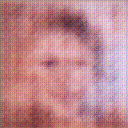
\includegraphics[width=150px]{500_fake_images/samples_5_390.png}%
\caption{A Close Up Of A Person With A Dog}%
\end{figure}

%
\end{document}